\documentclass[a4paper]{article}

\usepackage{mathrsfs}
% ============================================
%         General Packages
% ============================================
\usepackage{balance}

\usepackage{kotex}      % for Korean
\usepackage{lipsum}     % for dummy text
\usepackage{array}

\usepackage{cite}   % for citation

\usepackage{amsmath,amsfonts}
\usepackage{amssymb}
\usepackage{soul}
\usepackage{mathrsfs}

\usepackage{hyperref}

    \hypersetup{
        pdftoolbar=false,        	% show Acrobat’s toolbar?
        pdfmenubar=false,        	% show Acrobat’s menu?
        pdffitwindow=false,     	% window fit to page when opened
        pdfstartview={FitH},    	% fits the width of the page to the window
        pdftitle={},    	% title
        pdfauthor={},     	% author
        %     pdfsubject={},   	% subject of the document
        %     pdfcreator={},   	% creator of the document
        %     pdfproducer={}, 	% producer of the document
        %     pdfkeywords={keyword1, key2, key3}, % list of keywords
        %     pdfnewwindow=true,      	% links in new PDF window
        colorlinks=true,       	% false: boxed links; true: colored links
        linkcolor=blue,          	% color of internal links (change box color with linkbordercolor)
        citecolor=blue,       	% color of links to bibliography
        filecolor=blue,      	% color of file links
        urlcolor=blue		% color of external links
    }

\usepackage{algorithm}
\usepackage{algorithmic}

\usepackage{epsfig}
\usepackage[dvipsnames]{xcolor}

% MY PACKAGES ===================================

\usepackage{svg}
\usepackage{subfig}

\usepackage{textcomp}
\usepackage{stfloats}
\usepackage{url}
\usepackage{verbatim}
\usepackage{graphicx}
\usepackage{multirow}
\usepackage{multicol}

\let\proof\relax
\let\endproof\relax
\usepackage{amsthm}
\usepackage{lipsum}
\usepackage{tikz}

% 
\usepackage{titlepic}
\usepackage{pdfpages}
\usepackage{etoolbox} % 조건문을 쓰기 위한 패키지


\titlepic{%
  
\includegraphics[height = 8mm]{figures/logo_KAIST_simple.png}
  \hspace{5mm}
  
\includegraphics[height = 8mm]{figures/MIC_Logo.png}
  }

% ========================================
%         TITLE and AUTHORS
% ========================================
\title{
  Continual Model Learning
}

\author{
  \href{https://kaist-mic-lab.github.io/members/dhHong/}{Donghwa Hong}
}

\date{
    Compiled on \today
}

\begin{document}

\maketitle

% ========================================
%         Contents
% ========================================

% The cover image from the original Markdown is intentionally omitted.
\begin{figure}[h]
  \centering
  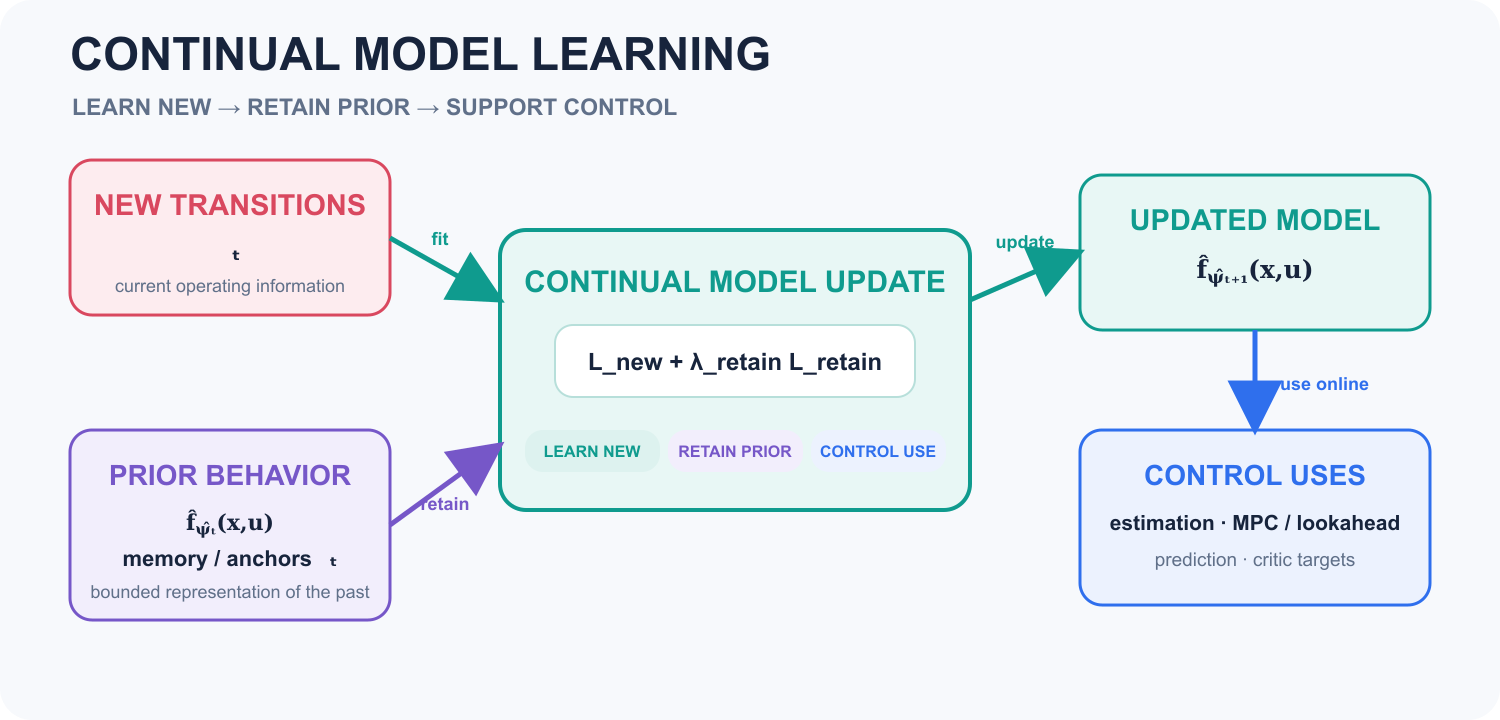
\includegraphics[width=\textwidth]{figures/05_continual_model_learning.png}
  \caption{Continual model learning fits new data while retaining prior model
  behavior.}
  \label{fig:continual_model_learning}
\end{figure}

Physical interaction is indexed by $k$, whereas learner updates are indexed
by $t$; the two clocks need not advance at the same rate.
$\widehat\psi_t$ denotes the model parameter available before update $t$, and
$\widehat\psi_{t+1}$ denotes the updated parameter.

\section{Problem definition}

\href{https://kaist-mic-lab.github.io/research/research_themes/00_online_learning_based_optimal_control/}{Online Learning-Based Optimal Control}
requires decision-state and successor information for Bellman-based control.
Continual Model Learning addresses the identifier/estimator-side problem:
learn a dynamics model from new real measurements without losing earlier
model behavior still needed by the estimator or controller.

Consider
\begin{equation}
  x_{k+1}=f(x_k,u_k,w_k),
  \qquad
  y_k=h(x_k)+v_k,
\end{equation}
where $x_k$, $u_k$, and $y_k$ are the state, control input, and measurement;
$f$ and $h$ are the state-transition and measurement maps; and $w_k$ and
$v_k$ represent process and measurement uncertainty. Unless a different
stochastic predictor is declared, the learned one-step target is the
conditional mean
\begin{equation}
  \overline f(x,u)
  :=
  \mathbb E[x_{k+1}\mid x_k=x,u_k=u]
  \approx
  \widehat f_{\widehat\psi_t}(x,u).
\end{equation}

The primary continual-learning scope is coverage expansion for a fixed
underlying predictor $\overline f$: new operating regions are added while
selected prior function behavior is retained. Genuine physical drift is a
different case. If the same $(x,u)$ acquires a different successor law because
of temperature, aging, load, or another condition, that condition should be
represented explicitly, for example by $\overline f(x,u;\eta)$, or handled by
a declared tracking/forgetting rule. Blind retention can otherwise preserve
obsolete behavior.

When both state and model are unknown, the basic identification principle is
measurement--dynamics consistency:
\begin{equation}
  \left(x_{0:k}^{\star},\psi^{\star}\right)
  \in
  \arg\min_{x_{0:k},\psi}
  \left\{
  \mathcal L_{\mathrm{meas}}(x_{0:k};y_{0:k})
  +
  \mathcal L_{\mathrm{dyn}}(x_{0:k},\psi;u_{0:k-1})
  \right\}.
\end{equation}

For example, quadratic measurement and dynamics residuals are
\begin{equation}
  \begin{aligned}
  \mathcal L_{\mathrm{meas}}(x_{0:k};y_{0:k})
  &=
  \sum_{i=0}^{k}
  \left\|y_i-h(x_i)\right\|_{W_y}^{2},\\
  \mathcal L_{\mathrm{dyn}}(x_{0:k},\psi;u_{0:k-1})
  &=
  \sum_{i=0}^{k-1}
  \left\|
  x_{i+1}-\widehat f_{\psi}(x_i,u_i)
  \right\|_{W_x}^{2},
  \end{aligned}
\end{equation}
where $W_y\succeq0$ and $W_x\succeq0$ weight the measurement and dynamics
residuals, respectively. An online implementation evaluates these losses over
a recent window rather than the entire trajectory.

Real measurements form the stream
\begin{equation}
  d_k=(y_k,u_k,y_{k+1}),
  \qquad
  \mathcal D_{0:k(t)-1}
  :=
  (d_0,\ldots,d_{k(t)-1}),
  \qquad
  \mathcal S_t\subseteq\mathcal D_{0:k(t)-1}.
\end{equation}

Here $k(t)$ is the latest measurement/state index available at learner update
$t$. The set $\mathcal S_t$ may contain only the latest completed transition
or a short selected history. If the state is directly measured, replace $y_k$
by $x_k$ and the problem reduces to model learning alone. Otherwise, the
latent state trajectory and model parameters must be estimated jointly, or a
separate estimator must supply $\widehat x_k$.

\section{Why this problem matters}

A model learned once offline may become incomplete as a mobility system visits
new loads, temperatures, road conditions, aging states, or operating regions.
Online system identification can reduce the residual on the newest trajectory,
but the updated function may no longer represent regions learned earlier.

This distinction matters because a controller does not query the model only at
the latest sample. State estimators, MPC or lookahead optimization, and critic
targets may evaluate it over many control-relevant states and inputs.
Continual learning therefore seeks both \textbf{new-region fit} and
\textbf{prior-function retention}, rather than only a small current residual.

\section{Key challenges}

\begin{itemize}
  \item \textbf{Limited and policy-dependent data:} real transitions arrive
  sequentially along the deployed closed-loop trajectory and do not freely
  cover the full state--input domain.
  \item \textbf{New learning versus prior-function retention}\\
  \textbf{(the stability--plasticity trade-off):} the learner must\\
  incorporate newly observed behavior without overwriting earlier behavior that
  remains relevant.
  \item \textbf{State--model coupling:} when $x_k$ is latent, state-estimation
  error and model error can explain the same residual and must be separated
  under suitable observability and excitation conditions.
  \item \textbf{Control-relevant online learning:} memory, update time,
  multistep error, model acceptance, and the effect of each update on
  downstream control matter in addition to one-step prediction loss.
\end{itemize}

\section{A conventional approach — recent-data residual minimization}

One conventional online-identification approach fits the model to the latest
transition or a short recent window. For notational simplicity, assume here
that the state is available; $x_j$ is replaced by $\widehat x_j$ when a
separate estimator is used:
\begin{equation}
  \begin{aligned}
  \widehat\psi_{t+1}
  &\approx
  \arg\min_{\psi}
  \mathcal L_{\mathrm{new}}(\psi;\mathcal S_t),\\
  \mathcal L_{\mathrm{new}}(\psi;\mathcal S_t)
  &:=
  \sum_{j\in\mathcal I_t}
  \left\|
  x_{j+1}-\widehat f_{\psi}(x_j,u_j)
  \right\|_{W_x}^{2}.
  \end{aligned}
\end{equation}

$\mathcal I_t$ indexes the recent transitions admitted to update $t$. This
update is useful for reducing current residuals, especially when the physical
dynamics truly change. Under limited excitation, however, it becomes a
trajectory-local online-identification update: it fits the currently visited
region but does not explicitly preserve model behavior learned in earlier
regions.

Tracking a genuinely changing model and retaining knowledge over an expanding
task domain are therefore different objectives and should be evaluated
separately.

\section{Research direction — function-retaining continual learning}

A continual formulation augments current measurement--dynamics consistency
with explicit retention of the previously learned function. Let
$k_t:=k(t)$ be the newest physical sample available at learner update $t$, and
let $M$ be the estimation-window length. The set $\mathcal S_t$ supplies the
transitions selected to fit newly observed behavior, whereas
$\mathcal M_t=\{(\bar x_\ell,\bar u_\ell)\}_{\ell=1}^{m_t}
\subseteq\mathcal X\times\mathcal U$ is a bounded set of state--input anchors
selected to retain prior model behavior. An anchor may be derived from a
transition in $\mathcal S_t$, but $\mathcal M_t$ can additionally contain
earlier stored points with pseudo-targets generated from the pre-update model:
\begin{equation}
  \begin{aligned}
  \left(
  \widehat x_{k_t-M:k_t},
  \widehat\psi_{t+1}
  \right)
  \approx
  \arg\min_{x_{k_t-M:k_t},\psi}
  \Big\{&
  \mathcal L_{\mathrm{meas},t}(x;\mathcal S_t)
  +
  \mathcal L_{\mathrm{dyn},t}(x,\psi;\mathcal S_t)\\
  &+
  \lambda_{\mathrm{retain}}
  \mathcal L_{\mathrm{retain}}
  \!\left(
  \widehat f_{\psi},
  \widehat f_{\widehat\psi_t};
  \mathcal M_t
  \right)
  \Big\}.
  \end{aligned}
\end{equation}

Here $\mathcal L_{\mathrm{meas},t}$ and
$\mathcal L_{\mathrm{dyn},t}$ are the residual losses defined in Section 1,
evaluated on $\mathcal S_t$. In a recent-window implementation,
$\mathcal S_t=\{d_j\mid j=k_t-M,\ldots,k_t-1\}$ supports the state and
measurement window ending at $k_t$. The retention weight satisfies
$\lambda_{\mathrm{retain}}\ge0$.

For example, functional retention over a bounded anchor set
$\mathcal M_t$ can be written as
\begin{equation}
  \mathcal L_{\mathrm{retain}}
  =
  \frac{1}{|\mathcal M_t|}
  \sum_{(\bar x,\bar u)\in\mathcal M_t}
  \left\|
  \widehat f_{\psi}(\bar x,\bar u)
  -
  \widehat f_{\widehat\psi_t}(\bar x,\bar u)
  \right\|_{W_r}^{2}.
\end{equation}

This expression assumes $|\mathcal M_t|>0$ and a positive-semidefinite weight
$W_r\succeq0$. If no anchors are retained, the retention term is omitted.

The first two losses explain current measurements and dynamics; the last loss
retains selected input--output behavior of the model available before the
update. If $x_k$ is measured, remove the state-trajectory decision and
$\mathcal L_{\mathrm{meas},t}$. The retention weight and anchor set define a
design trade-off; they do not guarantee global accuracy or eliminate
forgetting.

Candidate mechanisms include a small representative replay set, local or RBF
activation, pseudo-data generated from the previous model, and functional
regularization. These are candidate directions, not achieved MIC Lab results.

Future evidence should compare recent-only fitting, bounded-memory retention,
and full replay using new-region error, return-to-prior-region error,
multistep prediction, estimator error, downstream control performance, memory,
and update time.

\section{Application domains}

\begin{itemize}
  \item \textbf{Continual calibration of vehicle, electric-drive,}\\
  \textbf{energy-management, and thermal-system models} across operating
  regions and explicitly represented load, temperature, or aging conditions.
  \item \textbf{Control-oriented model learning for state estimation, MPC,
  online lookahead, and critic targets}, where the model must remain useful
  beyond the latest trajectory.
  \item \textbf{Model learning in complex real environments} where complete
  offline data and repeated full retraining are impractical.
\end{itemize}

\section{References}

\small
\begin{itemize}
  \setlength{\itemsep}{0pt}
  \setlength{\parskip}{0pt}
  \item D. Hong and K. Choi, \href{
  https://kaist-mic-lab.github.io/static/pub/2026-state-error-based-online-learning.pdf
  }{"State-Error-Based Online Learning of Control-Oriented Tire Force Models
  Using Grid Memory,"} ICROS, accepted, in press, 2026.
  \item D. Hong and K. Choi, \href{
  https://kaist-mic-lab.github.io/static/pub/2025-integral-error-based-adaptive.pdf
  }{"Integral Error-Based Adaptive Neural Identifier for Nonlinear Lateral
  Tire Forces,"} IEEE International Conference on Advanced Motion Control
  (AMC), pp. 1--6, 2026.
\end{itemize}

\end{document}
